\begin{ejercicio}
    % ID: 9
        Mostrar que $\overline{\alpha}*\alpha\simeq c_{x_1}\rel$.
    \end{ejercicio}

    \begin{demostracion}
        Sea la función continua $f:I\to I$ tal que
    \begin{align*}
    % La gráfica ahora va a la izquierda
    \vcenter{\hbox{
    \begin{tikzpicture}[scale=1.6]
        % Ejes sin etiquetas
        \draw[->, >=stealth] (-0.2, 0) -- (1.3, 0);
        \draw[->, >=stealth] (0, -0.2) -- (0, 1.3);
        % Marcas en los ejes (CON marca/rayita en 1/2)
        \draw (0.5, 1.5pt) -- (0.5, -1.5pt) node[below, font=\footnotesize] {$\nicefrac{1}{2}$};
        \draw (1, 1.5pt) -- (1, -1.5pt) node[below, font=\footnotesize] {$1$};
        \draw (1.5pt, 1) -- (-1.5pt, 1) node[left, font=\footnotesize] {$1$};
        % Gráfica de la función (color verde militar)
        \draw[thick, green!35!black] (0,1) -- (0.5,0) -- (1,1);
        % Puntos clave (vértices)
        \filldraw[green!35!black] (0,1) circle (1pt);
        \filldraw[green!35!black] (0.5,0) circle (1pt);
        \filldraw[green!35!black] (1,1) circle (1pt);
    \end{tikzpicture}
    }}
    \hspace{1cm} % Espacio de separación entre la gráfica y la ecuación
    f(s) &=
    \begin{cases} 
        1-2s, & \text{si } s\in [0,\nicefrac{1}{2}]; \\[1ex]
        2s-1, & \text{si } s \in [\nicefrac{1}{2},1].
    \end{cases}
    \end{align*}
    Se sigue que, $f\simeq c_{1}\rel$, entonces $\alpha\circ f\simeq {\alpha}\circ c_{1}\rel$. 
    dado que ${\alpha}\circ c_1=c_{x_1}$ y 
    \begin{align*}
        (\alpha\circ f)(s) &=
    \begin{cases} 
        \alpha(1-2s), & \text{si } s\in [0,\nicefrac{1}{2}]; \\[1ex]
        \alpha(2s-1), & \text{si } s \in [\nicefrac{1}{2},1].
    \end{cases}\\
    &=(\overline{\alpha}*{\alpha})(s)
    \end{align*}
    i.e., $\alpha\circ f=\overline{\alpha}*{\alpha}$. Por lo tanto, $\overline{\alpha}*{\alpha}\simeq c_{x_0}\rel$.
    \end{demostracion}
